\section{The forward-rate model}\label{sec:setting}
\subsection{Dates, rates, and bond prices}
We use $t$ for the date on which a curve is observed and $T$ for the maturity of a contract, with $0\le t\le T$. The instantaneous forward rate $f(t,T)$ is the rate observed at $t$ for an infinitesimal lending period starting at $T$. Its diagonal value $r_t=f(t,t)$ is the short rate. A zero-coupon bond paying one unit at $T$ has price
\begin{equation}
P(t,T)=\exp\left(-\int_t^T f(t,u)\dd u\right).
\label{eq:bonddefinition}
\end{equation}
Thus a change in the integral of the forward curve changes the logarithm of the bond price with the opposite sign. This relation is why the shape of the curve, rather than just its value at a few maturities, matters for consistency.

For statements on a particular calendar, fix a horizon $H>0$. Section~\ref{sec:realizations} explicitly quantifies over all finite horizons when asking for one realization serving every schedule. There are $N$ scheduled meetings, at deterministic dates $T_1,\ldots,T_N$. Set
\[
0=T_0<T_1<\cdots<T_N<H=T_{N+1},\qquad I_k=[T_k,T_{k+1}).
\]
The interval $I_k$ is the range of maturities between meetings $k$ and $k+1$; $T_0$ and $T_{N+1}$ are boundary dates, not additional meetings. At a given time $t<H$, let $j(t)$ be the unique index with $t\in I_{j(t)}$. We take values at interval endpoints from the right.

\subsection{Continuous changes and announcements}
Work on a filtered probability space with pricing measure $Q$. The information available at $t$ is $\F_t$; the information just before meeting $T_n$ is $\F_{T_n-}$. The filtration satisfies the usual conditions. Let $W$ be a vector of independent Brownian motions, representing continuously arriving shocks.

For each fixed maturity $T$, the initial rate is $f_0(T)$. Between meetings its drift is $\alpha(t,T)$ and its vector of Brownian sensitivities is $\sigma(t,T)$. At meeting $T_n$, define the announcement change
\[
\xi_n(T)=f(T_n,T)-f(T_n-,T),\qquad T\ge T_n.
\]
This is a random function of the remaining maturity $T$. With this notation the evolution is
\begin{equation}
f(t,T)=f_0(T)+\int_0^t\alpha(s,T)\dd s
 +\int_0^t\sigma(s,T)\cdot\dd W_s
 +\sum_{T_n\le t}\xi_n(T).
\label{eq:hjm}
\end{equation}
The four terms are the initial curve, accumulated drift, accumulated continuous shocks, and accumulated announcement changes. The dot denotes the Euclidean inner product. Coefficients have the measurability and local integrability required for these integrals; more specific conditions are stated with each result. We use the standard stochastic integral and It\^o formula; see \citet{revuz1999continuous}.

Figure~\ref{fig:discontinuities} distinguishes the two kinds of discontinuity. Holding $t$ fixed, the function $T\mapsto f(t,T)$ may have a break at a future meeting date $T_n$. It assigns different rates to periods before and after that meeting. Holding $T$ fixed instead, the function $t\mapsto f(t,T)$ may jump when the announcement arrives; that jump is $\xi_n(T)$.

For example, a curve can be flat at one rate before the next meeting and at another rate afterward, while both levels evolve continuously before the meeting. This curve has a maturity breakpoint. If every fixed-maturity rate also remains continuous through the meeting, then $\xi_n=0$, although the short rate can jump as it passes from the first interval to the second. That short-rate jump is known immediately before the date in the continuous-filtration models used below. Section~\ref{sec:jumps} studies nonzero announcement changes. Sections~\ref{sec:realizations}--\ref{sec:splice} set them to zero and study the dynamics of maturity breakpoints.

\begin{figure}[htbp]
\centering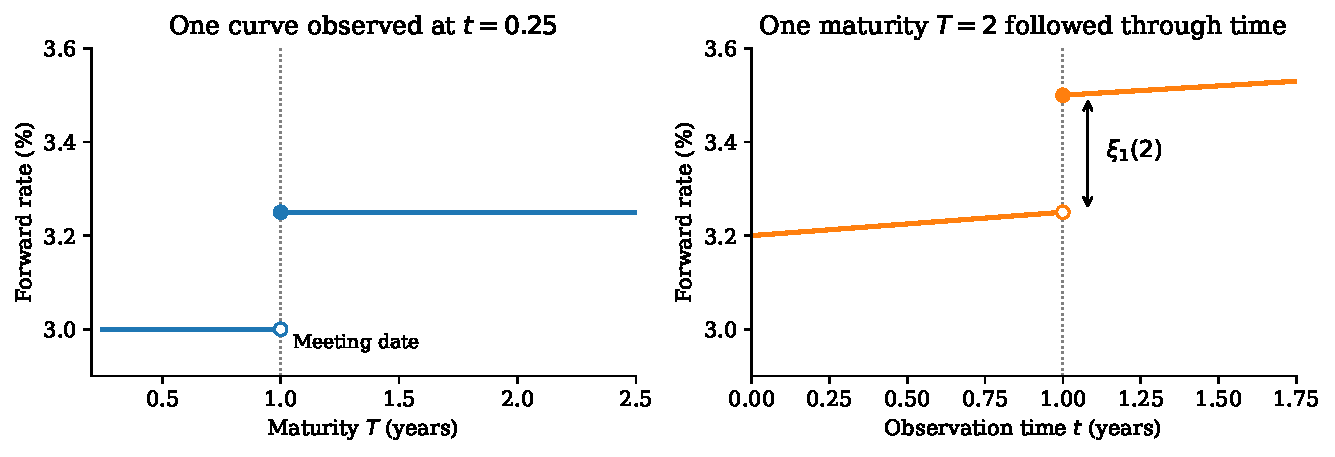
\includegraphics[width=\linewidth]{figures/two_discontinuities.pdf}
\caption{Two different meanings of a meeting-date discontinuity. Left: at one observation time, the forward curve assigns different rates to maturities before and after a future meeting. Right: for one fixed maturity, the rate changes when an announcement arrives. These are schematic illustrations of the two axes, not paths generated by a calibrated model.}\label{fig:discontinuities}
\end{figure}

\subsection{The restrictions imposed by bond prices}
The bank account is $B_t=\exp(\int_0^t r_s\dd s)$. Under the pricing measure, discounted bond prices $P(t,T)/B_t$ must have zero local drift. Between announcements, It\^o's formula applied to \eqref{eq:bonddefinition} gives the following restriction, the integrated form of the drift condition of \citet{heath1992bond}.

\begin{assumption}[Integrated drift condition]\label{ass:drift}
For every maturity $T$, for $Q\otimes dt$-almost every $(\omega,t)$ with $t\le T$,
\begin{equation}
\int_t^T\alpha(t,u)\dd u
 =\frac12\left|\int_t^T\sigma(t,u)\dd u\right|^2.
\label{eq:drift}
\end{equation}
\end{assumption}
The integral on the right is the bond's Brownian sensitivity, up to sign. Its squared norm supplies the It\^o correction. Thus volatility determines the integrated forward drift. Wherever maturity differentiation is valid, the equivalent pointwise formula is
\begin{equation}
\alpha(t,T)=\sigma(t,T)\cdot\int_t^T\sigma(t,u)\dd u.
\label{eq:diffdrift}
\end{equation}
This formula explains the elementary obstruction from the introduction. If $\sigma(t,T)=s$ is constant in maturity on an interval beginning at $t$, then $\alpha(t,T)=|s|^2(T-t)$ there. A constant volatility generates a sloping drift.

At an announcement, \eqref{eq:bonddefinition} gives the bond-price ratio
\[
\frac{P(T_n,T)}{P(T_n-,T)}
 =\exp\left(-\int_{T_n}^T\xi_n(u)\dd u\right).
\]
The bank account is continuous at $T_n$. The conditional expected bond-price ratio must therefore be one:
\begin{assumption}[Scheduled-jump condition]\label{ass:jump}
For every meeting $T_n$ and maturity $T\ge T_n$,
\begin{equation}
\E\left[\exp\left(-\int_{T_n}^T\xi_n(u)\dd u\right)
 \middle|\F_{T_n-}\right]=1\quad Q\text{-a.s.}
\label{eq:jump}
\end{equation}
\end{assumption}
Here $\E$ means expectation under $Q$. This is a restriction on the distribution of the entire integrated announcement change. Requiring only that the rate change have conditional mean zero would not suffice, because the exponential is nonlinear.

These two conditions specialize \citet[Theorem 3.5 and Remark 3.9]{fontana2022term} to the bond definition \eqref{eq:bonddefinition}, a continuous bank account, and finitely many deterministic announcement dates. In this paper, consistency means satisfaction of these conditions while remaining in the stated curve family. A true-martingale conclusion for discounted bonds additionally requires the corresponding integrability; local drift identities alone do not supply it.

\subsection{Curves that are linear between meetings}
The simplest extension of a curve that is flat between meetings allows a slope on each interval. For $T\in I_m$ write
\begin{equation}
f(t,T)=L_m(t)+C_m(t)(T-T_m),\qquad T\ge t.
\label{eq:front}
\end{equation}
The coefficient $L_m(t)$ is the level at the interval's left endpoint, and $C_m(t)$ is its slope as a function of maturity. A later interval has its own level and slope, so a break at a meeting is allowed. We denote this family by $S^+$ and its zero-slope subfamily by $S$.

In the diffusion models below, the levels have Brownian noise and the slopes have finite variation. Consequently volatility is constant in maturity on each interval, while drift can be linear there, as required by \eqref{eq:diffdrift}. Section~\ref{sec:splice} adds a smooth component to this piecewise-linear curve. We call the piecewise-linear component the \emph{front end} and the smooth component the \emph{block}; the sum is the \emph{splice}.

Equality of stochastic curve representations means almost-sure equality at each fixed $t,T$. For bond prices we use a jointly measurable maturity version, constructed in Section~\ref{sec:approximation}. The following elementary observation specifies the exceptional-set convention used in the drift proofs.

\begin{lemma}[A common exceptional set for maturities]\label{lem:maturitynull}
Suppose the drift and volatility are locally integrable in maturity and satisfy \eqref{eq:drift} for every fixed $T$, almost everywhere in time and probability. Then there is one time--probability exceptional set outside which the integrated identity holds for every $T\ge t$. If the drift and volatility are continuous inside each maturity interval, then for $T>t$, \eqref{eq:diffdrift} holds at every interior maturity outside that set.
\end{lemma}
\begin{proof}
Take the union of the exceptional sets for rational $T$, together with the set on which the maturity integrals fail to be defined. This is a null set. The primitives on both sides of \eqref{eq:drift} are continuous in $T$, so agreement on rational maturities extends to all maturities. On an interval with continuous coefficients, differentiation gives \eqref{eq:diffdrift} throughout its interior.
\end{proof}
